\documentclass[a4paper,12pt]{report}
\usepackage{algorithmic}
\usepackage[linesnumbered,ruled,vlined]{algorithm2e}
\usepackage[margin=2cm]{geometry}
\usepackage[utf8]{inputenc}
\usepackage{listings} 
\usepackage{graphicx} 
\usepackage{color}
\usepackage{xcolor}
\usepackage{hyperref}
\usepackage{subcaption}
\usepackage[bottom]{footmisc}
\usepackage{verbatim}
\usepackage{fancyvrb}
\usepackage{amsmath}
%\usepackage{mdframed}

\newcommand{\currentdata}{30 December 2019}
\newtheorem{example}{Example}

\begin{document}
\vspace{-5cm}
\begin{center}
Department of Computer Science\\
Technical University of Cluj-Napoca\\

\includegraphics[width=10cm]{fig/footer}
\end{center}
\vspace{1cm}
%\maketitle
\begin{center}
\begin{Large}
 %\textbf{Introduction to Artificial Intelligence}\\
\textbf{Introduction to Artificial Intelligence}\\
\end{Large}
\textit{Laboratory activity 2019-2020}\\
\vspace{3cm}
Project title:	Heuristic search\\
Tool: Pacman agent\\
\vspace{1.5cm}
Name: Mateiu Bianca\\
Group: 30434\\
Email: mateiu.bianca@gmail.com\\
\vspace{6cm}
%Assoc. Prof. dr. eng. Adrian Groza\\
%Adrian.Groza@cs.utcluj.ro\\
\vspace{1cm}

\includegraphics[width=10cm]{fig/footer}
\end{center}

\tableofcontents

\chapter{Installing the tool ($W_2$)}

The tool I have chosen to work with is \texttt{Pacman agent}, a tool developed by the Berkeley University, for their artificial intelligence course.\cite{wiki:04} Also, the operating system I have worked with is Windows 10, so the following instructions for installing the tool apply to this particular os.

Prior to installing the tool, one has to make sure the computer has the following prerequisites installed and working properly.

\label{l:requierements}
Firstly, verify that Python 2.7 is installed on the computer. It is important that the version is 2.7, because the tool is not compatible with any newer versions of python. To check the version simply run the Windows PowerShell, and type the command: \texttt{python --version}. If you do not have python installed, simply go to their website: \href{https://www.python.org/downloads/}{www.python.org/downloads/}, and search for a release version starting with 2.7. The next step is to download either the \textit{Windows x86-64 MSI installer} or the \textit{Windows x86 MSI installer}. After the download is complete, run the installer and follow the instructions it provides.

Secondly, it would be very helpful to have a dedicated IDE for python programming, or even just a code editor. Some good options are \textit{Atom, Visual Studio Code, Eclipse}. The IDE I used is \textit{PyCharm}, therefore I will give indications on using the tool in this environment. Of course, this step is not mandatory, since python files can be ran using the Windows command line, but int the case of projects having a large number of files, this dedicated IDE's make it easier to keep track of your work.

After making sure that this step is completed, we can proceed to installing the tool. In order to do this, one has to follow a few simple steps:

\begin{enumerate}
\item Go to Berekley's CS188 Introduction to AI \href{http://ai.berkeley.edu/search.html}{website}
\item Download the \textit{search.zip} archive containing the source code and supporting files
\item Extract the files to the preferred working directory
\item Launch PyCharm and go to \texttt{File -> Open}, and locate the directory you extracted the archive \textit{search.zip} to
\item In order to run the tool, we need to configure the project interpreter to Python 2.7, that you have already installed. For this, go to \texttt{File -> Settings}, and in the newly opened window, click on \texttt{Project -> Project Interpreter}. The next step is to choose from the dropdown list Python 2.7, or click on \textit{Show more...} if that option is not on the list. If you still can not find this option, than you must add a new Project Interpreter: click on the \textbf{+} sign, and locate the directory of the Python 2.7 executable file. 
\end{enumerate}

After following this steps, you should be able to use the tool: click right on the \textit{pacman.py} file and run it. A new window should open up, with the classical game of Pacman.

\chapter{Running and understanding examples ($W_3$)}

At a closer inspection of the files in this project, we will find a file called \textit{commands.txt} that contains a list of parameters that can be used to run the pacman program. This tool has many options, that can be studied by running the program with the \textit{-h} parameter. In order to supply this parameters to the program in PyCharm, we have to go to \texttt{Run -> Edit Configuration}, and type them in the \texttt{Parameters} input box. 

The most options we are going to use most often are:

\begin{itemize}
	\item \textit{-l} or \textit{-layout} followed by the name of a file found in the \textit{layouts} directory. This changes Pacman's environment, more precisely the maze.
	\item \textit{-p} or \textit{-pacman} followed by the name of the agent chooses the agent type that will be used.
	\item \textit{-a} or \textit{-agentArgs} followed by comma sepparated values represents the arguments that will be sent to the agent. This are often functions or heuristic to be used by the agent.
	\item \textit{-q} shuts down the graphical interface part of the tool
\end{itemize}

Before we continue, we should clarify the terms \textit{agent} and \textit{environment} and their meaning in the world of Artificial Intelligence. According to AIMA, "An \textbf{agent} is anything that can be viewed as perceiving its \textbf{environment} through sensors and acting upon that environment through actuators"\cite{russell2016artificial}.
Therefore, our pacman is in fact an agent, and its environment is the maze he finds himself into. 

Next, I will exemplify some of the capabilities of this tool:

\section{Classic pacman}
If we simply run the \textit{pacman.py} file, without any configuration, the classical game of Pacman will appear in a new window. You can even play the game: control it using the arrow keys.  Figure \ref{fig:pic1} shows a snapshot of the game.


In this example, Pacman is a Keyboard Agent. The implementation of this agent can be found in the file \textit{keyboardAgents}. Other agents are implemented in \textit{searchAgents.py}.

\section{West Agent}
By using the configuration:

\vspace{0.3cm}
\fbox{\begin{minipage}{16cm}
 \texttt{--layout testMaze --pacman GoWestAgent}    
\end{minipage}}
\vspace{0.3cm}

we can see how another Pacman agent behaves. This is a fairly simple agent, and all it does is go west. See \ref{fig:pic1}. 
Of course, when we are dealing with more imbricated layouts that require turning to get to the goal, this agent will fail.\ref{wiki:04}

\section{Search Agent}
In order to use this tool to its full potential, we have no interest in using an agent that we have to control, or that is capable of one thing only, as we did before. That is why in this example we will be using the Search Agent, that is fully implemented for us and can be found in the file \textit{searchAgents.py}. For this, you will be using the following configuration:

\vspace{0.3cm}
\fbox{\begin{minipage}{16cm}
 \texttt{-l tinyMaze -p SearchAgent -a fn=tinyMazeSearch}    
\end{minipage}}
\vspace{0.3cm}

You will notice that this search agent also receives a function that it will use in navigating the maze: \textit{tinyMazeSearch} (found in \textit{search.py}). This function simply hardcodes the solution for one particular maze. This function describes the behaviour of the agent. (See \ref{fig:pic1})


\vspace{0.5cm}
\begin{figure}[h!]
  \centering
  \begin{subfigure}[b]{0.6\linewidth}
    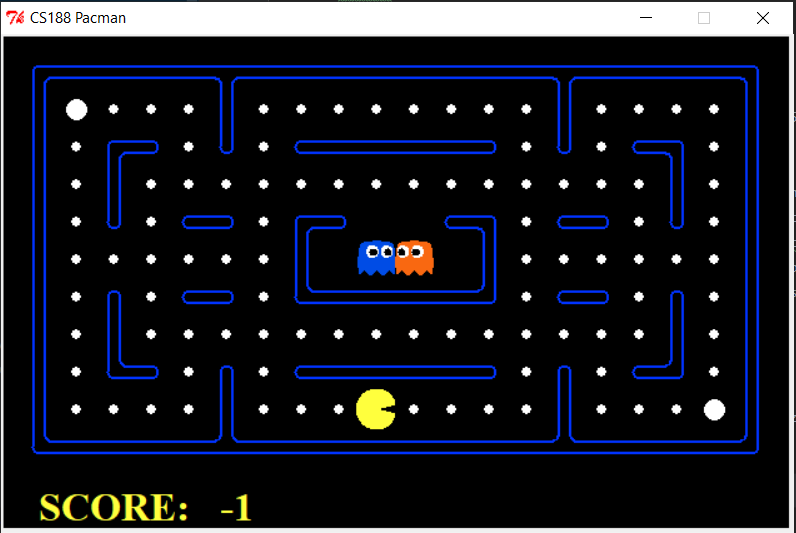
\includegraphics[width=\linewidth]{pictures/pacman.png}
    \caption{A game of Pacman.}
  \end{subfigure}
  \begin{subfigure}[b]{0.4\linewidth}
    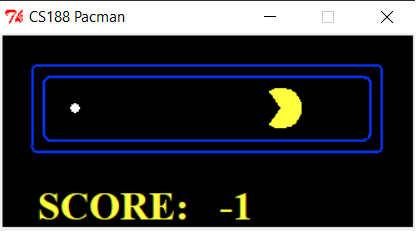
\includegraphics[width=\linewidth]{pictures/pacman2.png}
    \caption{West Agent.}
  \end{subfigure}
\hspace{0.5cm}
	\begin{subfigure}[b]{0.3\linewidth}
    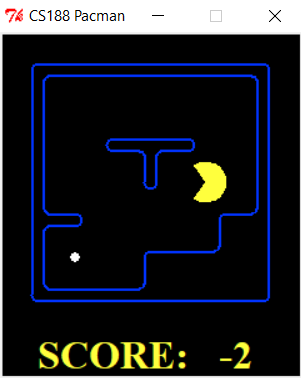
\includegraphics[width=\linewidth]{pictures/pacman3.png}
    \caption{Search Agent.}
  \end{subfigure}
  \caption{Different Pacman configurations}
  \label{fig:pic1}
\end{figure}

\vspace{0.5cm}

 
\chapter{Understanding conceptual instrumentation ($W_4$)}

The tool has many functioning modes, that can be controlled by the means of the sent parameters. For example, you could have training games for Pacman, or record the results.

The next algorithm describes the main part of the tool, the runGames function:


\begin{algorithm}
\label{alg:eval}
\caption{Run Games.}

\KwIn{\textit{layout} - an object containing information about the maze, such as the position of walls, food and agents;\\
	\textit{pacman} - the search agent;\\
	\textit{ghosts} - a list of ghost agents;\\
	\textit{display} - an object containing information about the graphicla interface of the game;\\
	\textit{numGames} - the number of games to play;\\
	\textit{record} - save game data to a file;\\
	\textit{numTraining} - the number of episodes that are training(surpess output);\\
	\textit{catchException} - turns on exception handling during games;\\
	\textit{timeout} - maximum time an agent can spend computing in a game;\\
}
\KwOut{\textit{games} - a list of all the ran games}

{$games \leftarrow$ empty list}\\
\For{$i\leftarrow$ 2 $\KwTo$ $numGames$}{
	{$beQuiet \leftarrow (i \geq numTraining)$}

	\eIf {beQuiet}
	{surpress output and graphics}
	{$gameDisplay \leftarrow display$}

	{$game \leftarrow$ newGame()}\\
	{$game$.run()}

	\If {! beQuiet}
		{$games \leftarrow games + game$}

	\If {record}
		{save data to file}
}
\If {numGames - numTraining $\geq$ 0}
	{print statistics of the games}

{return $games$}

\end{algorithm}



\chapter{Project description ($W_5$)}

\section{Narrative description}

I plan on using this tool to experiment with different searching algorithms, and see how different algorithms behave in terms of optimality and time complexity with a given problem. The problem is the following: start from an initial position in a maze and reach a goal position in the minimum number of steps, and with the minimum number of explored states (therefore, in the smallest amount of time).

The search problem has been extensively discussed before, and dozens of algorithms have been developed to solve it. Also, it can be easily translated into real life problems: finding a route from a town to another, planning a trip by taking into consideration transportation, finding a path through a maze (like in Pacman), finding solutions for games that have a finite set of states, transitions and one single goal (such as eight puzzle). More that that, the pathfinding problem is one of the most popular AI problem in the rising industry of computer games, where often this problem has to be solved in real time, and with limited resources of memory and CPU resources. \cite{wiki:05}

Therefore, I will implement a number of searching algorithms I find suitable for the task, use the tool to run them multiple times on randomly generated mazes of various sizes, store the data, then query and manipulate it and record my findings.

\section{Facts}
I will consider two searching strategies:
\begin{enumerate}
	\item uninformed search
	\item informed search
\end{enumerate}

I will start with uniformed search first. This are algorithms that only use the information provided to them by the problem. They can distinguish a non-goal state from a goal state, but they can not tell if one state is closer to the goal than another, therefore if that state should be prioritized. Whereas, informed search algoritms can, and use heuristics an priority queues in order to do that. \cite{russell2016artificial}

The uninformed search algorithms that I will take into consideration are \textit{Breadth First Search, Depth First Search, Uniform Cost Search, Bidirectional Search}. The informed search algorithms that I will take into consideration are \textit{Astar} and \textit{Dynamic Weighting Astar}. Also, as an heuristic for the informed search, I will be using the classical Manhattan distance, and I will also develop my own heuristic, appropriate for the maze problem.

\section{Specifications}
In my approach of using the Pacman tool, the input parameters will be the following ones: a Position search problem, and a function that is to be used to solve that problem. There will be a number of functions, some using heuristics, some not. The relevant information that can be found in the problem is:
\begin{itemize}
	\item a list containing information about the grid's cells, which contain a wall and which don't. This information will be read and processed from a layout file
	\item the staring position in the grid
	\item the goal
	\item the number of explored states, or, in other words, the number of visited cells
\end{itemize}

In regards to the output of the program, we will not be concerned with the grapihical capabilities of the tool, so we will only take into consideration the information about the performance of the searching algorithm used, namely the cost of the found solution and the number of expanded nodes. This information will be stored in a .csv file, and manipulated later on, after the program has been ran on a large enough set of input data (layouts and functions) so that the result will have credibility. 

Moreover, another objective I have set is to learn using another tool that will help me manipulate the data and transform it into charts, so that the conclusion is easier to draw. I will be using \textit{Jupyter Notebook} for this, along with the libraries \textit{Pandas} and \textit{Matplotlib}.


\section{Knowledge acquisition}

\paragraph{How do represent knowledge?} 

The knowledge my system requires is a simple layout file, conatining a perfect maze, represented by symbols such as '\textit{\%}' for walls and spaces for hallways. The initial position and goal also have to be represented: with '\textit{P}' and '\textit{.}'. Of course, in order to see which algorithms find the optimal solution (minimum cost) and which don't, there should be more than one path between start and destination.

\paragraph{Where are you getting the required knowledge/data}
I used an algorithm\cite{wiki:02} that creates a perfect maze\footnote{"A so called 'perfect' maze has every path connected to every other path, so there are no unreachable areas. Also, there are no path loops or isolated walls. There is always one unique path between any two points in the maze." \cite{wiki:03}}, and which is based on the Depth first search algorithm. I adjusted the algorithm in order to obtain a layout compatible with the Pacman tool, and made the maze not be a perfect one, since we do not want that.


\section{Related work}
There are hundreds of papers that can be found on the subject of search problems. The one source of inspiration and knowledge that I used more than others is the book \textit{Artificial Intelligence A Modern Approach}\cite{russell2016artificial}

\section{Assumptions}
My assumptions are that informed search will prove to be quicker to reach the goal first, but that this will sometimes happen at the expense of not always finding the optimal solution. 



\chapter{Implementation details ($W_9$)}


As I have mentioned before, my approach to this project is a rather experimental one. I focused on researching the strong and weak point of informed and uninformed search strategies, and as a result, this project does not model on a particular real life situation. Despite this, the route finding problem is something people face every day, and my findings can be easily translated in a real life scenario.

This being said, since I am using the Pacman tool, my project is based on developing search algorithms that are meant to help Pacman find its way through the maze.

\section{Relevant code}

\subsection{Searching algorithms}

The algorithms I implemented in this project can be divided into two categories:

\begin{enumerate}
	\item uninformed search:
		\begin{itemize}
			\item Breadth First Search
			\item Depth First Search
			\item Uniform Cost Search
			\item Bidirectional Search
		\end{itemize}
	\item informed search:
		\begin{itemize}
			\item Astar
			\item Dynamic Weighting Astar
		\end{itemize}
\end{enumerate}

I have also created a \textit{Node} structure, where I store the information about each state the Search Agent finds himself into. This structure has a general implementation, so that it can be used in other problems, not just the \textit{Position search problem}. The \textit{Node} class has the following fields:

\begin{itemize}
	\item state - the current state
	\item cost - the cost of getting to this state
	\item action - a list of the necessary actions to get to this state
	\item parent - the Parent node
	\item depth - the length of the path from the current node to the starting node
\end{itemize}

The \textit{Node} class also has a method, \textit{getNeighbors}, that uses the problem to generate the list of states that can be reached from the current state

I will now briefly explain every algorithm:

\paragraph{Breadth First Search} is a simple strategy in which the root node is expanded first, then all the successors of the root node are expanded next, then their successors, and so on. In general, all the nodes are expanded at a given depth in the search tree before any nodes at the next level are expanded. The data structure used for the frontier is the Queue (LIFO). \cite{russell2016artificial}

\paragraph{Depth First Search} always expands the \textit{deepest} node in the frontier. The data structure used for the frontier is the Stack (FIFO). \cite{russell2016artificial}

\paragraph{Uniform Cost Search} is similar to the BFS algorithm, but instead of using a queue to store the frontier nodes, UCS uses a priority queue, to make sure that the nodes with the lowest path cost are expanded first.

\paragraph{Bidirectional Search} can be used for problems where we know both the initial position and the goal. The idea is to run two BFS algorithms, one from the initial state and one from the goal, and build the solution when the frontier of this 2 algorithms intersect. \cite{russell2016artificial}

\paragraph{Astar} is a form of BFS, but the evaluating function of the nodes is different:

\vspace{0.3cm}
\fbox{\begin{minipage}{16cm}
 \texttt{$f(n) = g(n) + h(n)$}    
\end{minipage}}
\vspace{0.3cm}

where g(n) is the cost to reach the node, and h(n) is the cost to get to the goal. \cite{russell2016artificial} H(n) is an heuristic function, and depending on this function, we can improve this algorithm even further.


\paragraph{Dynamic Weighting Astar} is a form of the Astar algorithm that uses dynamic weights for the heuristic function. The idea in this algorithm is that at the beginning, it is important to get anywhere fast, so the heuristic, or the approximated cost to get to the goal is not as important. But as the nodes increase in depth, the heuristic becomes more and more important. So, the function evaluating the nodes becomes:

\vspace{0.3cm}
\fbox{
\parbox{16cm}{
{$f(n) = g(n) + (1 + \sigma * w(n)) * h(n)$,\\
where 
\[
    w(n)=
\begin{cases}
    {1 - \frac{d(n)}{N}},& \text{if } d(n)\le N\\
    0,              & \text{otherwise}
\end{cases}
\]
and $d(n)$ is the depth of the search and $N$ is the anticipated length of the solution path
}
}}
\vspace{0.3cm}\cite{wiki:01}

I used two different heuristics for the informed search strategies: the Manhattan Distance, and an heuristic developed by me, that combines the Manhattan Distance value with the number of walls found between the current state and the goal state. I tried this heuristic in multiple forms, by changing the weight of the walls number.


\subsection{Maze generation}

Another algorithm I used is the one that randomly generates the maze layouts, and it is based on the Depth first search algorithm.\cite{wiki:02}

The idea is to start with a grid of cells having all the walls between them. Then choose a random location from where to start the DFS algorithm. For each cell, mark it as visited, choose a random neighbor, and if it is not visited, remove the adjacent wall and continue the DFS with this node.

This algorithm generates a perfect maze (a maze in which for each 2 cells, there is a single path between them), but since we need to have more than one possible path from Pacman to the goal, we choose a number of random walls from the ones left and remove them.

Lastly, the string of the generated maze is written to a file.

\subsection{Generating graphs}

And last but not least, I used the online environment \textit{Jupyter Notebook}, and the libraries \textit{pandas} and \textit{matplotlib} to interpret the results. 

I configured the Pacman tool to run all the search algorithms on the same maze, and write the results in a .csv file. Then, in Jupyter Notebook, i used \textit{Pandas} to parse the data and save it into a structure called \textit{Data frame}, that enabled me to easily manipulate it. The next step was to use \textit{matplotlib}, a plotting library for python, to generate line graphs and bar graphs.

To give you an example of the capabilities of this tool, the graph in figure \ref{fig:pic2} was generated by the following piece of code:

\begin{verbatim} 
import pandas as pd
import matplotlib.pyplot as plt
%matplotlib inline

data = pd.read_csv("C:/Users/Bianca/Desktop/resultsSmall.csv")

df = pd.DataFrame(data)
barAll = pd.DataFrame(data, columns=['Function', 'Cost', 'Expanded'])
                 .groupby('Function')
                 .sum()
                 .sort_values(by = ['Expanded', 'Cost'], ascending=True)

barAll.plot(kind='barh')
\end{verbatim}

\begin{figure}[h!]
   \centering
    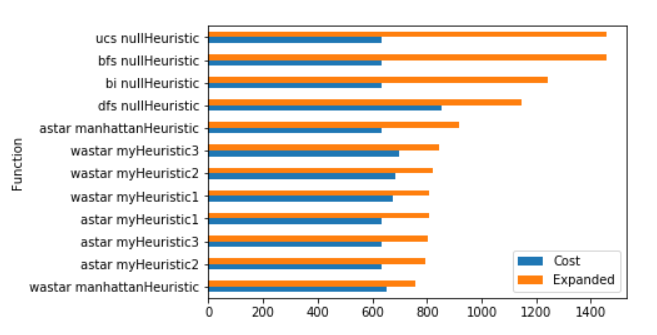
\includegraphics[width=\linewidth]{pictures/small/small1.png}
    \caption{The results registered by the program ran on small sized mazes}
  \label{fig:pic2}
\end{figure}
\vspace{0.5cm}

In the above code, I used pandas to create the data frame \textit{df}. Now, we have to manipulate this data frame in order to have the desired structure to display the graph. So, in the variable \textit{barAll}, I selected only the relevant collumns: \textit{Function, Code} and \textit{Expanded}. Using the function \textit{groupby} I grouped the data by the collumn \textit{Function}, and the values in the rest of the collumns are summed, and then sorted ascendingly by the \textit{Expanded} collumn and the \textit{Cost} collumn. After all this has been done, the data can be plotted.

\chapter{Tool expressivity ($W_{10}$)}

This tool can be used for more than just for a Pacman game. It gives the user the possibility to use it with diferent Search Agents and different Search Problems. So essentially, if a route finding problem can be described in terms of a Search Problem, than it can be solved by this tool.

\paragraph{The game} is the main part of this tool. There are also some \textit{GameRules}, where the definitions of winning and losing can be found. The game also defines the layout of the maze, the Search Agent, the Ghosts Agents, and other parameters meant to configure the game.

\paragraph{The Search Agent} receives a search algorithm and a search problem, and returns actions to follow for a path from an initial state and a goal (defined in a problem)

\paragraph{The Search Problem} defines the state space, start state, goal test, successor function and cost function. For example, for the Pacman game, the state space consists of (x, y) positions in a pacman game. For the eightpuzzle, the states are defined by different arrangements of the 8 digits.

\paragraph{The Ghost Agent} is another type of Agent, but instead of searching a path to a specific goal, it simply roams the maze.

In my program, I changed the configuration of the Search Agent, in order to provide it with different search algorithms to use.


\chapter{Graphs and experiments ($W_{11}$)}

My approach was the following: divide the experiment by the size of the maze. This way, I defined 4 classes of mazes:

\begin{enumerate}
\item small maze (16 x 8)\ref{fig:pic3}
\item medium mazes (40 x 20)\ref{fig:pic3}
\item large mazes (60 x 30)\ref{fig:pic3}
\item extra large mazes (80 x 40)\ref{fig:pic3}
\end{enumerate}

\vspace{0.5cm}
\begin{figure}[h!]
  \centering
  \begin{subfigure}[b]{0.4\linewidth}
    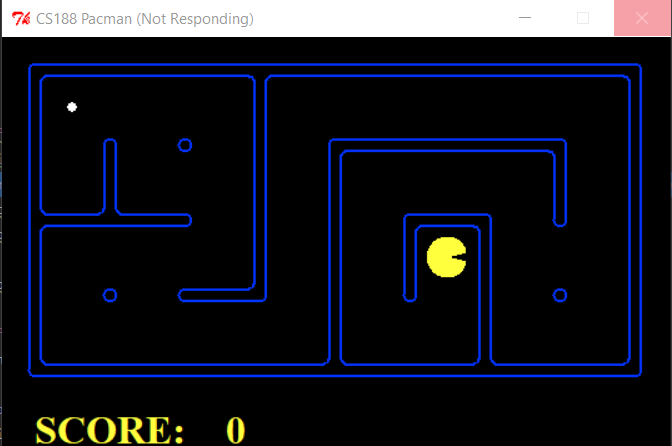
\includegraphics[width=\linewidth]{pictures/mazeSizes/small.png}
    \caption{Small.}
  \end{subfigure}
  \begin{subfigure}[b]{0.4\linewidth}
    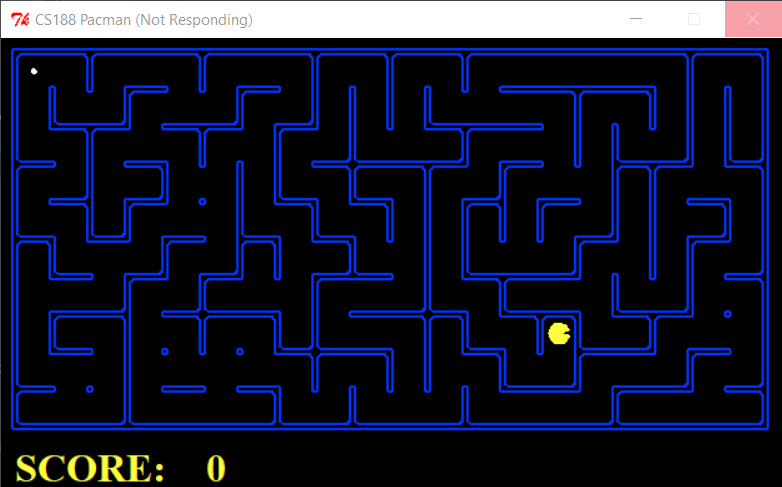
\includegraphics[width=\linewidth]{pictures/mazeSizes/medium.png}
    \caption{Medium.}
  \end{subfigure}
 \begin{subfigure}[b]{0.4\linewidth}
    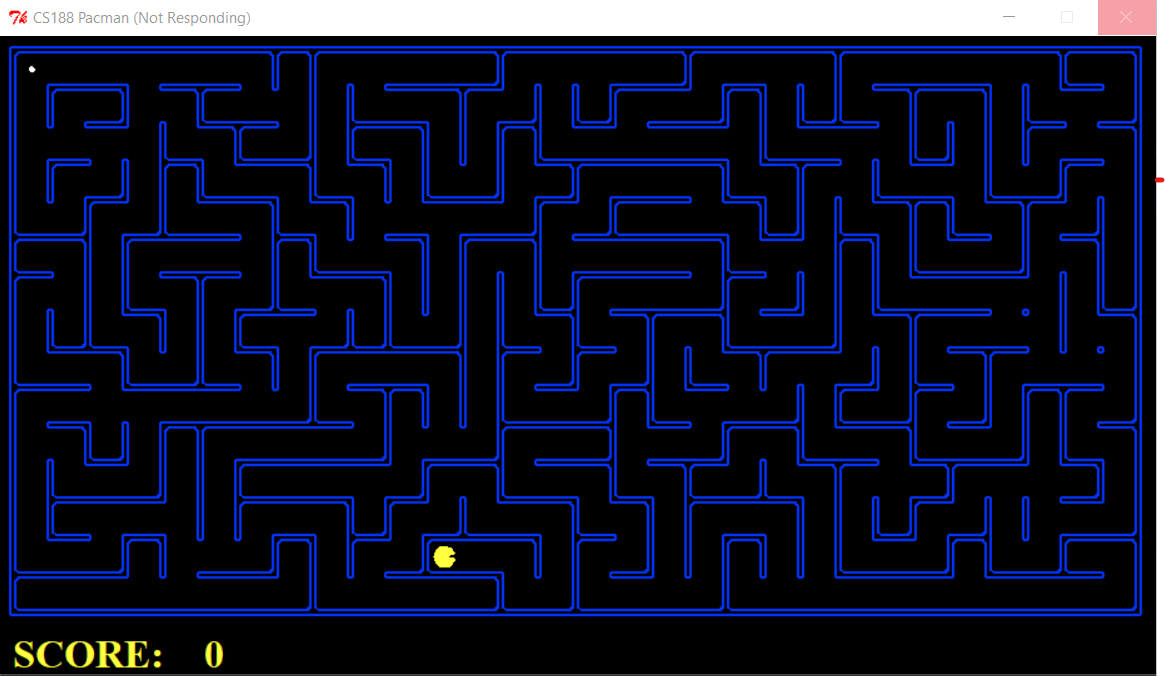
\includegraphics[width=\linewidth]{pictures/mazeSizes/large.png}
    \caption{Large.}
  \end{subfigure}
  \begin{subfigure}[b]{0.4\linewidth}
    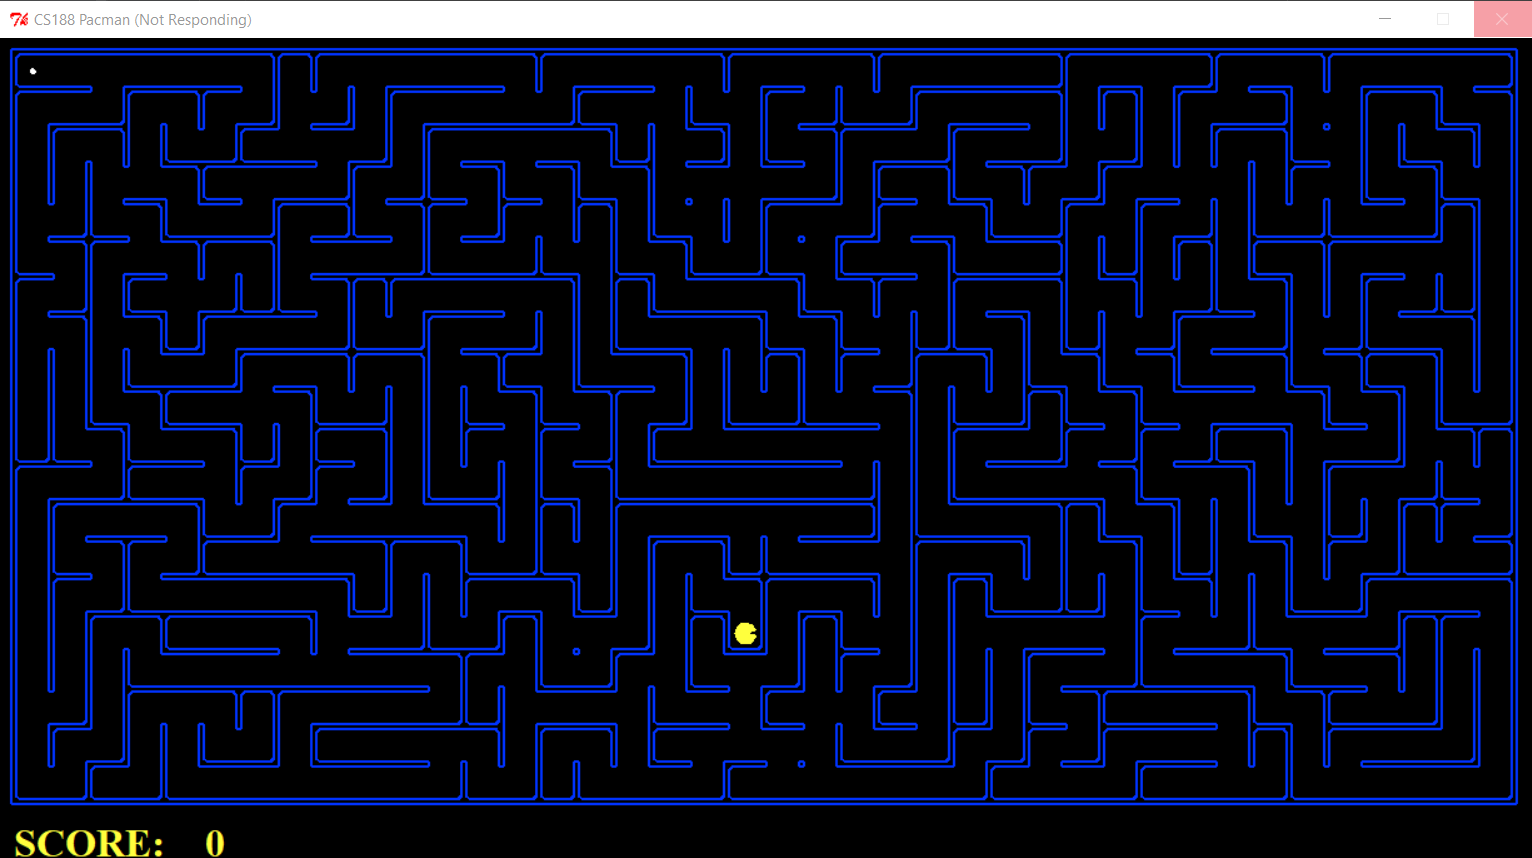
\includegraphics[width=\linewidth]{pictures/mazeSizes/extraLarge.png}
    \caption{Extra Large.}
  \end{subfigure}
  \caption{Maze Sizes}
  \label{fig:pic3}
\end{figure}

\vspace{0.5cm}

Since the maze layout is a random one, I would not obtain trust worthy results if I only ran the game once for each search algorithm. So, for each of this maze classes, I ran the program 30 times on 30 different layouts, for each of the 6 search algorithms. More than that, I wanted to test the informed search strategies with different heuristics. So I ran a different version of Astar and Weighted Astar, with the following heuristics: 

\begin{enumerate}
\item Manhattan Distance Heuristic
\item the heuristic I defined, weighing in the number of walls between the position and goal with a weight of 1
\item the heuristic I defined, weighing in the number of walls between the position and goal with a weight of 2
\item the heuristic I defined, weighing in the number of walls between the position and goal with a weight of 3
\end{enumerate}

Therefore, for each layout I ran 12 algorithms.

The output I recorded was the \textit{Cost} of the found path and the number of nodes that were \textit{Expanded} to get to the goal.

The results I obtained were, in some ways, what I expected them to be:

\vspace{0.5cm}
\begin{figure}[h!]
  \centering
  \begin{subfigure}[b]{0.45\linewidth}
    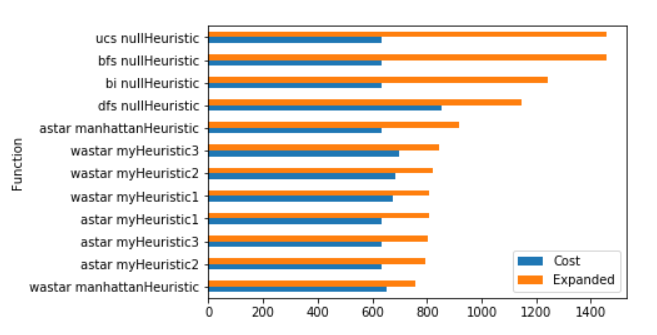
\includegraphics[width=\linewidth]{pictures/small/small1.png}
    \caption{Cost and Explored for Small mazes.}
  \end{subfigure}
  \begin{subfigure}[b]{0.45\linewidth}
    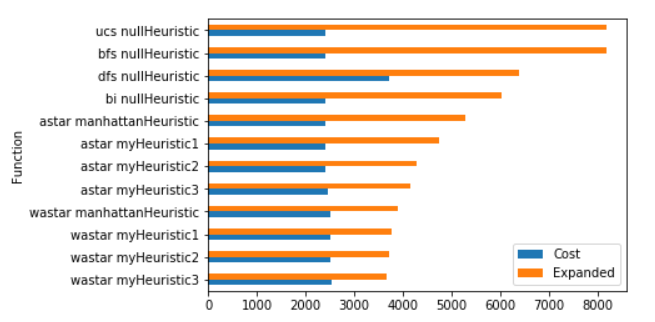
\includegraphics[width=\linewidth]{pictures/medium/small1.png}
    \caption{Cost and Explored for Medium mazes.}
  \end{subfigure}
 \begin{subfigure}[b]{0.45\linewidth}
    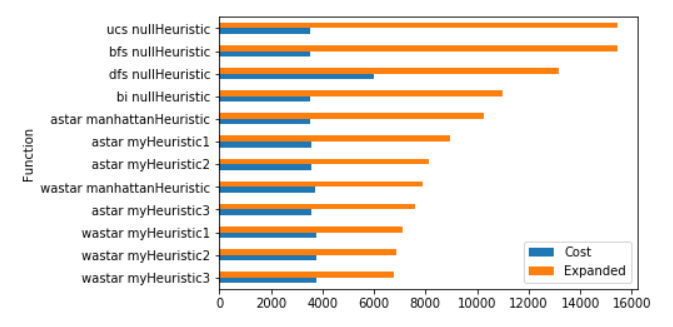
\includegraphics[width=\linewidth]{pictures/large/small1.png}
    \caption{Cost and Explored for Large mazes.}
  \end{subfigure}
  \begin{subfigure}[b]{0.45\linewidth}
    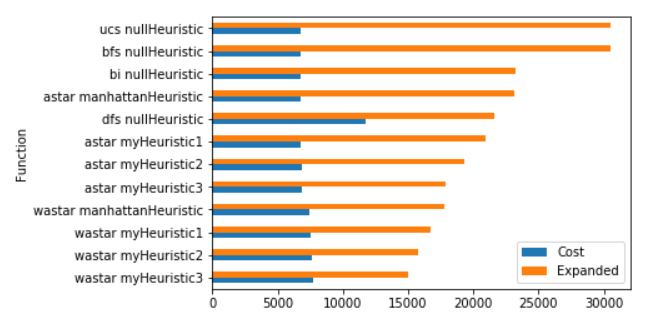
\includegraphics[width=\linewidth]{pictures/extraLarge/small1.png}
    \caption{Cost and Explored for Extra large mazes.}
  \end{subfigure}
  \caption{Results}
  \label{fig:pic4}
\end{figure}
\vspace{0.5cm}

And for a more precise analysis, here are the values based on which the previous graphs were generated:

\vspace{0.5cm}
\centerline{
\begin{minipage}{10cm}
\begin{tabular}{ccc}
Results for small mazes:\\
\hline
Function & Cost & Expanded \\
\hline
wastar manhattanHeuristic & 652 & 756\\
\hline
astar myHeuristic 2 & 632 & 794\\
\hline
astar myHeuristic 3 & 636 & 805\\
\hline
astar myHeuristic 1 & 632 & 808\\
\hline
wastar myHeuristic 1 & 676 & 809\\
\hline
wastar myHeuristic 2 & 684 & 823\\
\hline
wastar myHeuristic 3 & 700 & 843\\
\hline
astar manhattanHeuristic & 632 & 917\\
\hline
dfs & 852 & 1147\\
\hline
bi & 632 & 1243\\
\hline
bfs & 632 & 1458\\
\hline
ucs & 632 & 1458\\
\hline
 \end{tabular}
\vspace{0.2cm}
\end{minipage}
}
\vspace{0.5cm}

\centerline{
\begin{minipage}{10cm}
\begin{tabular}{ccc}
Results for medium mazes:\\
\hline
Function & Cost & Expanded \\
\hline
wastar myHeuristic 3 & 2540 & 3663\\
\hline
wastar myHeuristic 2 & 2512 & 3713\\
\hline
wastar myHeuristic 1 & 2508 & 3761\\
\hline
wastar manhattanHeuristic & 2520 & 3901\\
\hline
astar myHeuristic 3 & 2448 & 4145\\
\hline
astar myHeuristic 2 & 2404 & 4276\\
\hline
astar myHeuristic 1 & 2404 & 4752\\
\hline
astar manhattanHeuristic & 2396 & 5289\\
\hline
bi & 2396 & 6031\\
\hline
dfs & 3716 & 6395\\
\hline
bfs & 2396 & 8192\\
\hline
ucs & 2396 & 8192\\
\hline
 \end{tabular}
\vspace{0.2cm}
\end{minipage}
}
\vspace{0.5cm}

\centerline{
\begin{minipage}{10cm}
\begin{tabular}{ccc}
Results for large mazes:\\
\hline
Function & Cost & Expanded \\
\hline
wastar myHeuristic 3 & 3776 & 6748 \\
\hline
wastar myHeuristic 2 & 3756 & 6885 \\
\hline
wastar myHeuristic 1 & 3764 & 7088 \\
\hline
astar myHeuristic 3 & 3568 & 7597 \\
\hline
wastar manhattanHeuristic & 3700 & 7897 \\
\hline
astar myHeuristic 2 & 3548 & 8137 \\
\hline
astar myHeuristic 1 & 3548 & 8959 \\
\hline
astar manhattanHeuristic & 3532 & 10255 \\
\hline
bi & 3532 & 10966 \\
\hline
dfs & 5996 & 13150 \\
\hline
bfs & 3532 & 15456 \\
\hline
ucs & 3532 & 15456\\
\hline
 \end{tabular}
\vspace{0.2cm}
\end{minipage}
}
\vspace{0.5cm}

\centerline{
\begin{minipage}{10cm}
\begin{tabular}{ccc}
Results for extra large mazes:\\
\hline
Function & Cost & Expanded \\
\hline
wastar myHeuristic 3 & 7738 & 15029 \\
\hline
wastar myHeuristic 2 & 7650 & 15808 \\
\hline
wastar myHeuristic 1 & 7578 & 16708 \\
\hline
wastar manhattanHeuristic & 7398 & 17791 \\
\hline
astar myHeuristic 3 & 6882 & 17900 \\
\hline
astar myHeuristic 2 & 6818 & 19319 \\
\hline
astar myHeuristic 1 & 6766 & 20913 \\
\hline
dfs & 11786 & 21615 \\
\hline
astar manhattanHeuristic & 6762 & 23161 \\
\hline
bi & 6762 & 23270 \\
\hline
bfs & 6762 & 30532 \\
\hline
ucs & 6762 & 30532\\
\hline
 \end{tabular}
\vspace{0.2cm}
\end{minipage}
}
\vspace{0.5cm}


In terms of optimality (\textit{Cost}), the BFS algorithm is the best in all 4 cases. This was expected, since by the nature of this algorithm, it always finds the shortest path between a root and any other node. But the number of the \textit{Expanded} nodes registered by this algorithm is significantly higher than other algorithms.

The UCS algorithm behaves exactly like the BFS algorithm in this case. It is possible we would have seen an improvement in terms of the number of the expanded nodes, if the cost of actions in the maze were different than 1.

The Bidirectional BFS also finds the optimal path, and the number of expanded nodes is lower than the one registered by BFS, so we can already see an improvement.

The Depth First Search algorithm is the one that registeres the worst \textit{Cost} number. Combined with the still high number of Expanded nodes, I consider this the worst choice of search algorithm for this kind of problem.

As we have already noticed, the uninformed search strategies tend to explore a number of nodes that is almost double to the one of the informed search strategies. But they do find the shortest path (except for DFS).

Moving over to the informed search strategies, we notice that for small sized mazes, the Astar algorithm gives a better number of expanded nodes than the Weighted Astar. We can argue than since the path to the goal is shorter, it doesn't matter as much in the beginning to get \textit{anywhere}, as fast as possible, as the Weighted Astar behaves. And is more important to move in the general direction of the goal. But, if we consider the Cost of the path, Astar is closer to the optimal solution in all 4 scenarios. 

Also, we have to take into consideration the heuristic that has been used. We can observe that as the size of the maze increases, the Manhattan Distance heuristic becomes less and less useful, and the heuristic I defined proves itself to be better. From this we conclude that the number of walls we approximated to be between the position and the goal becomes more of an important factor as we are dealing with bigger sized mazes. And more than this, the heuristic using the weight = 3 (meaning that the number of walls is multiplied by 3, and then added to the Manhattan distance between points) is the one that leads to the lowest number of expanded nodes.

Another scenario I considered is one in which the size of the maze varies. The parameters in which the program was ran remain the same: I generated a random layout, and ran the 12 algorithms on this maze. The experiment was repeated 30 times, and the results were recorded. They can be seen in the following charts.

\begin{figure}[h!]
  \centering
  \begin{subfigure}[b]{0.45\linewidth}
    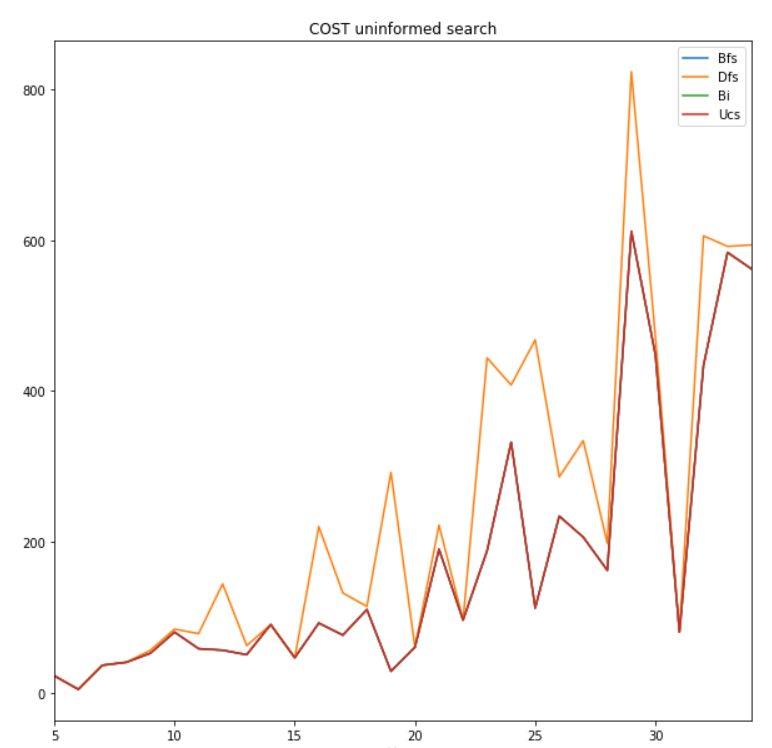
\includegraphics[width=\linewidth]{pictures/variedMazeSize/4.png}
    \caption{Cost - uninformed search}
  \end{subfigure}
  \begin{subfigure}[b]{0.45\linewidth}
    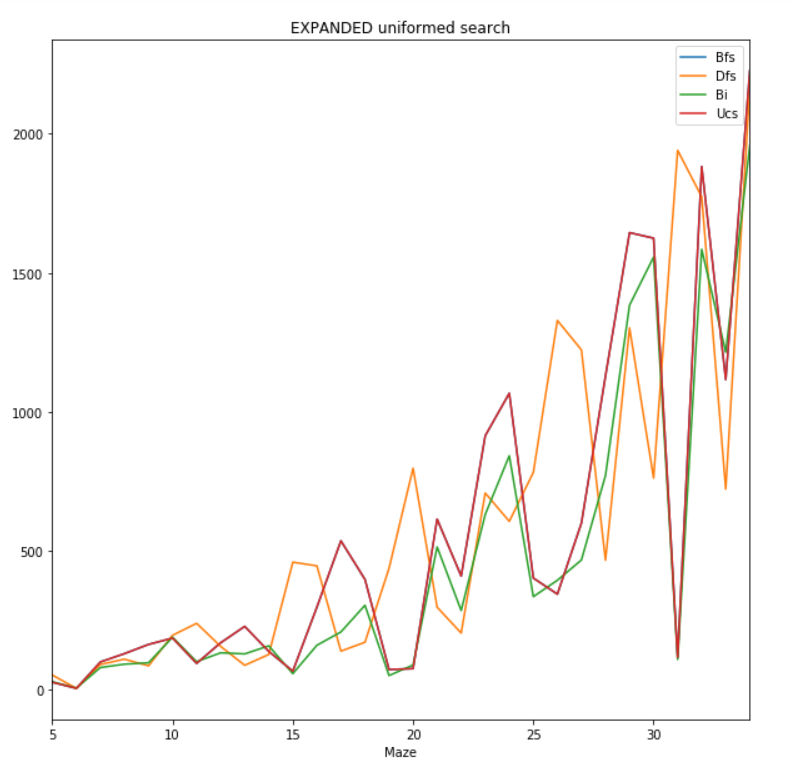
\includegraphics[width=\linewidth]{pictures/variedMazeSize/3.png}
    \caption{Explored nodes - uninformed search}
  \end{subfigure}
 \begin{subfigure}[b]{0.45\linewidth}
    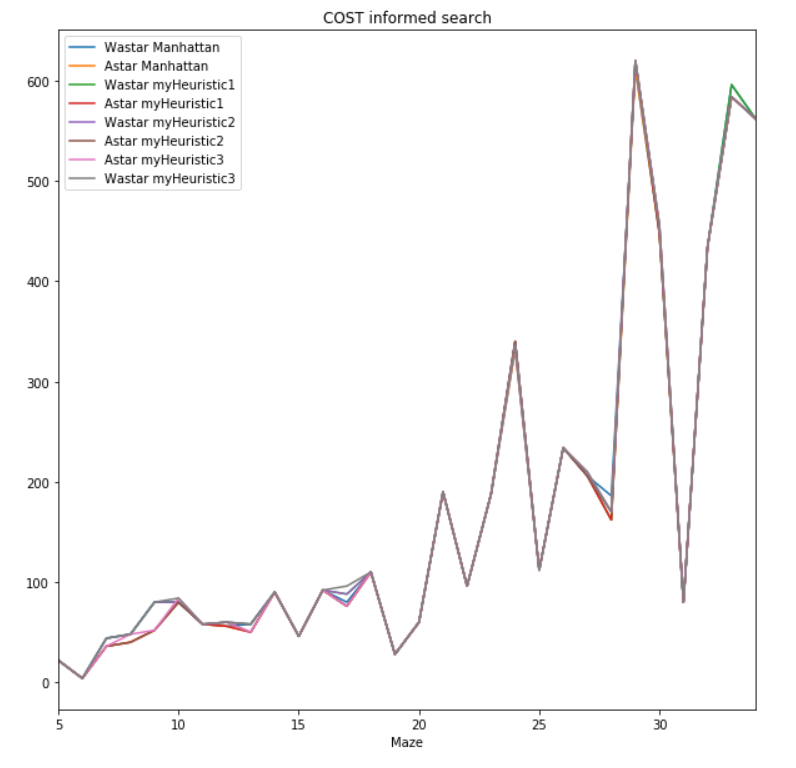
\includegraphics[width=\linewidth]{pictures/variedMazeSize/5.png}
    \caption{Cost - informed search}
  \end{subfigure}
  \begin{subfigure}[b]{0.45\linewidth}
    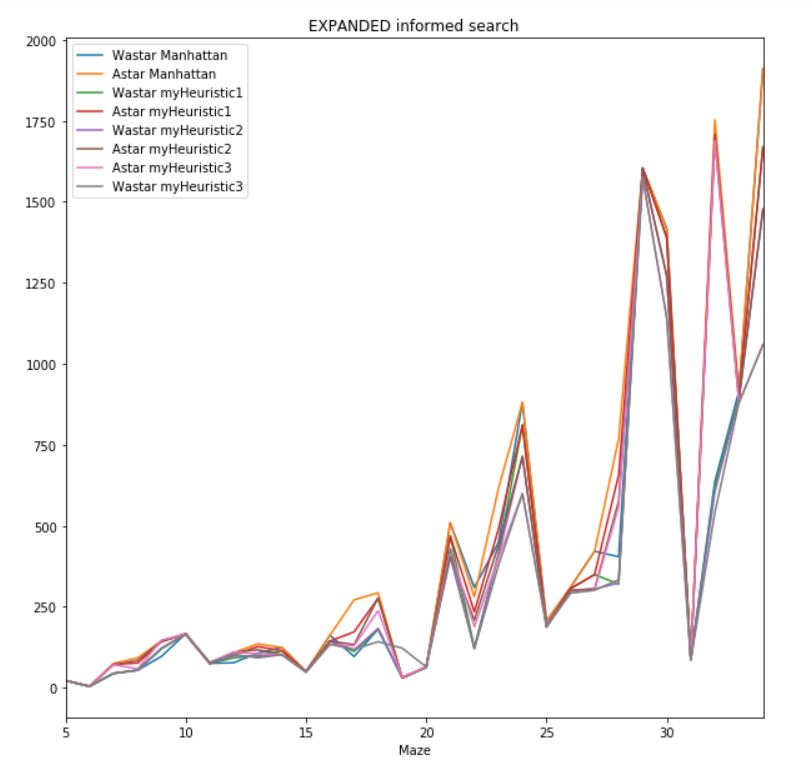
\includegraphics[width=\linewidth]{pictures/variedMazeSize/6.png}
    \caption{Explored nodes - informed search}
  \end{subfigure}
  \caption{Results - varying maze size}
  \label{fig:pic5}
\end{figure}
\vspace{0.5cm}

As expected, the path cost and number of explored nodes increase with the increase of the maze size.

My conclusion after the observations of this experiment is that when deciding what search algorithm to use in a position search problem, one must first ask what does one value more. If it is more important to find the lowest cost path, than an uninformed cost strategy, such as BFS or UCS is recommended. If instead it is more important to get to the goal with the lowest number of explored states, than it is worth looing into informed search strategy. And in order to get the best performance, the used function and heuristic can be decided dynamically at runtime, based on the size of the maze.

\chapter{Related work and documentation ($W_{12}$)}

My results are similar to other results from papers I have found on the subject. It is wildly accepted that the Astar algorithm is one of the best algorithms to use for the pathfinding problem, and it is to this day used in the world of computer games. For example, this paper\cite{wiki05}, Pathfinding in strategy games and maze solving using A search algorithm, describes its use in strategy games, and how this algorithm is considered to be an efficient and inexpensive approach.

I also found other works describing even more search algorithms, such as Maze Solving Algorithms, Paintbrush Algorithm, Breadth First Search Algorithm, Depth First Search Algorithm, Trimming Algorithm and Compass Algorithm\cite{wiki06}. This paper was particularly interesting, since it describes some algorithms developed by the authors. The one that is the highlight of the whole paper is the so called \textit{Paintbrush algorithm}, which is similar in concept to the floodfill in paintbrush (if you color a figure, any space that has contact to the figure will be colored). So, if you consider that you have a maze, each time you have to choose between going left or right, first close the right way, and fill the current cell with paint. If the goal cell is filled with paint as well, it means that by going to the left, you will surely find the path to the goal. If the goal cell is not painted, than the path, if there exists one, must be to the right.

Of course, I also used as guiding the book \textit{Artificial intelligence: a modern approach}\cite{russell2016artificial}, which I found to be great help in clarifying AI concepts and in documenting about the chosen search strategies.

\appendix

\chapter{Your original code}
\label{app:code}
This section should contain only code developed by you, without any line re-used from other sources. 
This section helps me to correctly evaluate your amount of work and results obtained. 
Including in this section any line of code taken from someone else leads to failure of IS class this year.
Failing or forgetting to add your code in this appendix leads to grade 1.
Don't remove the above lines.

\section{Heuristic function}

\begin{Verbatim}[frame=single]
def myHeuristic(position, problem, info={}):

    xy1 = position
    xy2 = problem.goal
    manhattan = abs(xy1[0] - xy2[0]) + abs(xy1[1] - xy2[1])
    xmin = min(xy1[0], xy2[0])
    xmax = max(xy1[0], xy2[0])
    ymin = min(xy1[1], xy2[1])
    ymax = max(xy1[1], xy2[1])

    list1 = problem.walls.data[xmax][ymin:ymax + 1]
    list2 = problem.walls.data[xmin][ymin:ymax + 1]
    list3 = [el[ymin] for el in problem.walls.data[xmin + 1:xmax]]
    list4 = [el[ymax] for el in problem.walls.data[xmin + 1:xmax]]
    count = list1.count(True) + list2.count(True) 
                + list3.count(True) + list4.count(True)
    count /= 2

    return manhattan + int(problem.heuristicWeight) * count
\end{Verbatim}

\section{Node class}

\begin{Verbatim}[frame=single]
class Node:
    def __init__(self, state, cost=0, action=None, parent=None, depth=0):
        self.state = state
        self.cost = cost
        if action is None:
            self.action = []
        else:
            self.action = action
        self.parent = parent
        self.depth = depth

    def __repr__(self):
        return "<Node %s>" % (self.state,)

    def getNeighbors(self, problem):
        neighbors = []
        for node in problem.getSuccessors(self.state):
            neighbors.append(node)
        return neighbors
\end{Verbatim}

\section{Breadth First Search}
\begin{Verbatim}[frame=single]
def breadthFirstSearch(problem):
    from util import Queue

    start = Node(problem.getStartState())
    explored, frontier = [], Queue()
    frontier.push(start)

    while not frontier.isEmpty():
        node = frontier.pop()
        if problem.isGoalState(node.state):
            return node.getAction()
        if node.state not in explored:
            explored.append(node.state)
            for child in node.getNeighbors(problem):
                if child[0] not in explored and child[0] not in frontier.list:
                    actions = node.getAction()[:]
                    actions.append(child[1])
                    frontier.push(Node(child[0],
                                        node.cost + child[2], actions, node))
    return []
\end{Verbatim}

\section{Depth First Search}

\begin{Verbatim}[frame=single]
def depthFirstSearch(problem):
    from util import Stack

    start = Node(problem.getStartState())
    explored, frontier = [], Stack()
    frontier.push(start)

    while not frontier.isEmpty():
        node = frontier.pop()
        if problem.isGoalState(node.state):
            return node.getAction()
        explored.append(node.state)
        for child in node.getNeighbors(problem):
            if child[0] not in explored and child[0] not in frontier.list:
                actions = node.getAction()[:]
                actions.append(child[1])
                frontier.push(Node(child[0],
                             node.cost + child[2], actions, node))
    return []
\end{Verbatim}

\section{Uniform Cost Search}

\begin{Verbatim}[frame=single]
def uniformCostSearch(problem):
    from util import PriorityQueue

    start = Node(problem.getStartState())
    explored, frontier = [], PriorityQueue()
    frontier.push(start, start.getPathCost())

    while not frontier.isEmpty():
        node = frontier.pop()
        if problem.isGoalState(node.state):
            return node.getAction()
        if node.state not in explored:
            explored.append(node.state)
            for child in node.getNeighbors(problem):
                if child[0] not in explored:
                    actions = node.getAction()[:]
                    actions.append(child[1])
                    childNode = Node(child[0],
                                     node.cost + child[2], actions, node)
                    frontier.update(childNode, childNode.getPathCost())
    return []
\end{Verbatim}

\section{Bidirectional Search}

\begin{Verbatim}[frame=single]
def computePath(nodeS, nodeG):
    actionsStart = nodeS.getAction()
    actionsGoal = nodeG.getAction()
    actualActionGoal = []
    for action in actionsGoal[::-1]:
        if action == 'South':
            actualActionGoal.append('North')
        if action == 'North':
            actualActionGoal.append('South')
        if action == 'East':
            actualActionGoal.append('West')
        if action == 'West':
            actualActionGoal.append('East')
    return actionsStart + actualActionGoal

def bidirectionalSearch(problem):
    from util import Queue

    start = Node(problem.getStartState())
    goal = Node(problem.getGoalState())
    explored, frontier1, frontier2 = [], Queue(), Queue()
    frontier1.push(start)
    frontier2.push(goal)

    while not frontier1.isEmpty() and not frontier2.isEmpty():
        if not frontier1.isEmpty():
            node1 = frontier1.pop()
            if node1.state == goal.state:
                return node1.getAction()
            if node1.state in (item.state for item in frontier2.list):
                for node in frontier2.list:
                    if node.state == node1.state:
                        return computePath(node1, node)
            if node1.state not in explored:
                explored.append(node1.state)
                for child in node1.getNeighbors(problem):
                    if child[0] not in explored:
                        actions = node1.getAction()[:]
                        actions.append(child[1])
                        frontier1.push(Node(child[0], 
                                             child[2], actions, node1))
        if not frontier2.isEmpty():
            node2 = frontier2.pop()
            if node2.state == start.state:
                return node2.getAction()
            if node2.state in (item.state for item in frontier1.list):
                for node in frontier1.list:
                    if node.state == node2.state:
                        return computePath(node, node2)
            if node2.state not in explored:
                explored.append(node2.state)
                for child in node2.getNeighbors(problem):
                    if child[0] not in explored:
                        actions = node2.getAction()[:]
                        actions.append(child[1])
                        frontier2.push(Node(child[0],
                                            child[2], actions, node2))

    return []
\end{Verbatim}

\section{Astar Search}

\begin{Verbatim}[frame=single]
def aStarSearch(problem, heuristic=nullHeuristic):
    from util import PriorityQueue

    start = Node(problem.getStartState())
    explored, frontier = [], PriorityQueue()
    frontier.push(start, start.cost)

    while not frontier.isEmpty():
        node = frontier.pop()
        if problem.isGoalState(node.state):
            return node.getAction()
        if node.state not in explored:
            explored.append(node.state)
            for child in node.getNeighbors(problem):
                if child[0] not in explored:
                    actions = node.getAction()[:]
                    actions.append(child[1])
                    childNode = Node(child[0],
                                 node.cost + child[2], actions, node)
                    frontier.update(childNode, 
                               childNode.getPathCost() + 
                               heuristic(childNode.state, problem))
    return []
\end{Verbatim}

\section{Weighted Astar Search}

\begin{Verbatim}[frame=single]
def weightedAStarSearch(problem, heuristic=nullHeuristic):
    from util import PriorityQueue
    from searchAgents import manhattanHeuristic

    start = Node(problem.getStartState())
    explored, frontier = [], PriorityQueue()
    frontier.push(start, start.cost)

    N = manhattanHeuristic(start.state, problem)

    sigma = 4

    while not frontier.isEmpty():
        node = frontier.pop()
        if problem.isGoalState(node.state):
            return node.getAction()
        if node.state not in explored:
            explored.append(node.state)
            for child in node.getNeighbors(problem):
                if child[0] not in explored:
                    actions = node.getAction()[:]
                    actions.append(child[1])
                    childNode = Node(child[0], node.cost + child[2], actions,
                                                 node, node.depth + 1)
                    if childNode.depth > N:
                        weight = 1
                    else:
                        weight = 1 + (1 - childNode.depth / N) * sigma
                    cost = childNode.getPathCost()
                              + weight * heuristic(childNode.state, problem)
                    frontier.update(childNode, cost)
    return []
\end{Verbatim}

\section{Generation of graphs}
\label{code:01}
\begin{Verbatim}[frame=single]
import pandas as pd
import matplotlib.pyplot as plt
%matplotlib inline

data = pd.read_csv("C:/Users/Bianca/Desktop/resultsSmall.csv")

df = pd.DataFrame(data)
barAll = pd.DataFrame(data, columns=['Function', 'Cost', 'Expanded'])
                 .groupby('Function')
                .sum()
                .sort_values(by = ['Expanded', 'Cost'], ascending=True)
barCost = pd.DataFrame(data, columns=['Function', 'Cost'])
                   .groupby('Function')
                   .sum()
                   .sort_values(by = ['Cost'], ascending=True)
barExpanded = pd.DataFrame(data, columns=['Function', 'Expanded'])
                            .groupby('Function')
                            .sum()
                            .sort_values(by = ['Expanded'], ascending=True)

barAll.plot(kind='barh')
barCost.plot(kind='barh')
barExpanded.plot(kind='barh')
\end{Verbatim}


\chapter{Quick technical guide for running your project}

The requirements and the instructions on installing the tool have already been specified: \ref{l:requierements}

Step by step technical manual:

\begin{enumerate}
\item open the file \textit{pacman.py}
\item depending on which type of maze size you want to run the problem, the parameters of the function \textit{generateMaze} will have to be changed. The values for each category can be found commented in the lines above the function definition
\item run the program
\item the results will be saved to a .csv file on the computer's Desktop
\end{enumerate}

In order to generate the graphs, you must first install \textit{Jupyter, Pandas} and \textit{Matplotlib}. I am using the python manager package, pip. To install them with pip, open a terminal window and type:

\begin{Verbatim}[frame=single]
    pip install jupyterlab
    pip install matplotlib
    pip install pandas
\end{Verbatim}

After the instalation, open a new terminal window and type \texttt{jupyter notebook} and create a new Notebook. You can use the code provided by me in the code section \ref{code:01}, and generate the graphs based on the data from the .csv file.



\bibliographystyle{plain}
\bibliography{is}


\vspace{2cm}
\begin{center}
Intelligent Systems Group\\

\includegraphics[width=10cm]{fig/footer}
\end{center}



\end{document}
